\chapter{Revisão de Literatura}
% \chapterprecis{}
\begin{quote}\normalfont\itshape\vspace*{-2\baselineskip}
  Neste capítulo inicialmente é
  apresentado o conceito de aprendizado ativo e um método de implementação.
  Em seguida é apontado o {\clicker} como uma
  ferramenta para ajudar o professor implementar o aprendizado significativo  em
  sala de aula. O capítulo é encerrado apresentando os benefícios e desafios de uso de dessa tecnologia.
\end{quote}


\section{Aprendizado Ativo}\label{section:aprendizado_ativo}
Método pedagógico que envolve os estudantes no aprendizado, de maneira bastante simples
essa é a definição de aprendizado ativo. Em resumo, aprendizado ativo é qualquer coisa
que além de envolver os estudantes no fazer, os faça pensar no que estão fazendo \cite[p. 19]{Charles1991}.

Os princípios do aprendizado ativo são dois: introduzir atividades nas salas de aula
tradicionais e promover o envolvimento dos estudantes. O primeiro é a forma
mais simples do aprendizado ativo. Um exemplo seria fazer pequenas pausas na aula
e colocar os estudantes para revisar as notas de aula com um colega. No entanto,
é preciso que tais atividades promovam o engajamento dos estudantes no processo
de ensino e aprendizagem \cite[p. 3]{Prince2004}.
% Métodos ativos como Instrução
% pelos Colegas \cite{} ...\footnote{colocar outros métodos ativos e resultados}

Em salas de aula que utilizam o aprendizado ativo pode-se ter um aumento de até 6\%
na média final nas provas dos alunos e que aquelas salas de aula puramente expositivas
têm 55\% mais chance de reprovarem os alunos do que aquelas com aprendizado ativo.
Esse aumento que pode parecer pouco (0,3 na média final) colocaria a média daqueles estudantes
que desistem do curso bem próximo daqueles que permanecem, podendo-se dessa forma aumentar
a taxa de retenção dos estudantes \cite[p. 4]{Freeman2014}.

O estudo de meta-análise de \citeonline{Freeman2014} envolveu mais de 200 artigos
que comparavam as performances dos alunos em salas de aula com pelo menos algum
elemento de aprendizado ativo com as tradicionais aulas expositivas. Além de
mostrarem evidências de que o aprendizado ativo pode melhorar o aprendizado dos
estudantes de graduação principalmente nas áreas de ciência, tecnologia, engenharia
e matemática, \citeauthoronline{Freeman2014} propõem aos futuros pesquisadores
testarem não mais a eficiência dos métodos de aprendizado ativo frente as tradicionais
aulas expositivas (``primeira geração de pesquisas''), mas sim de verificar qual
o tipo de aprendizado ativo é mais apropriado para cada área do conhecimento
(``segunda geração de pesquisas'').

No entanto, tornar o aluno um agente ativo no processo de ensino e aprendizagem dado a realidade brasileira
não é uma tarefa fácil. Muitas são as adversidades de infraestrutura e institucionais
encontradas de modo a propiciar uma aprendizagem significativa. Seja por salas com
numero excessivo de alunos, estes desinteressados, professores mal pagos, ou com
a pressão de produzir cientificamente \cite{Araujo2013}.

Por outro lado, muitas são as iniciativas encontradas na literatura mostrando resultados
satisfatórios que podem ajudar o professor nesse processo \cite{Crouch2001, Gok2013, Barros2004}.
Na próxima seção será apresentado o método ativo de ensino \textit{Peer Instruction} ou \textit{Instrução pelos Colegas}
(IpC)\nomenclature{IpC}{Instrução pelos Colegas}.

\subsection{Instrução pelos Colegas (IpC)}
\label{section:ipc}

O IpC foi desenvolvido pelo Professor Eriz Mazur da Universidade de Harvard (EUA)\nomenclature{EUA}{Estados Unidos da América} na
década de 1990. O objetivo do IpC é fazer com que todos os estudantes se engajem em
discussões com o vizinho de opinião diferente sobre um determinado conceito e fazer com que cada
estudante tente explicar o conceito um para o outro \cite{Mazur2009}.

No método IpC geralmente o professor começa fazendo uma breve exposição dialogada do conteúdo (15min).
Depois é colocado para os estudantes uma questão conceitual, que é
desenvolvida de modo a avaliar o entendimento dos estudantes sobre um tópico. Um
exemplo de uma questão conceitual de introdução a física é mostrada na \autoref{fig:desenv_ct}. Os
estudantes então individualmente respondem a questão (1-2min) geralmente utilizando
\textit{clickers}, que são pequenos dispositivos transmissores como os da \autoref{fig:desenv_clickers}.

Em seguida, dependendo do percentual de alunos que acertem a questão,
o professor pode revisar o assunto (acerto < 30\%), fazer uma breve explanação da
questão e ir para um próximo tópico ou nova questão (acerto > 70\%), ou o que se
deseja do método, um percentual de acerto entre 30\% e 70\% em que nessa situação o
professor estimula que os alunos encontrem um parceiro que respondeu preferencialmente de forma diferente
e que tentem explicar um para o outro o porquê de estar correto, ou seja, os alunos se auto
instruem temos então o nome do método ``Instrução pelos Colegas'' \cite{Mazur2009, Crouch2001}.
A \autoref{fig:desen_fluxograma_ipc} resume o processo de implementação do método IpC na sala de aula.

\begin{figure}[!htb]
  \centering
  \caption{Exemplo de uma questão conceitual}
  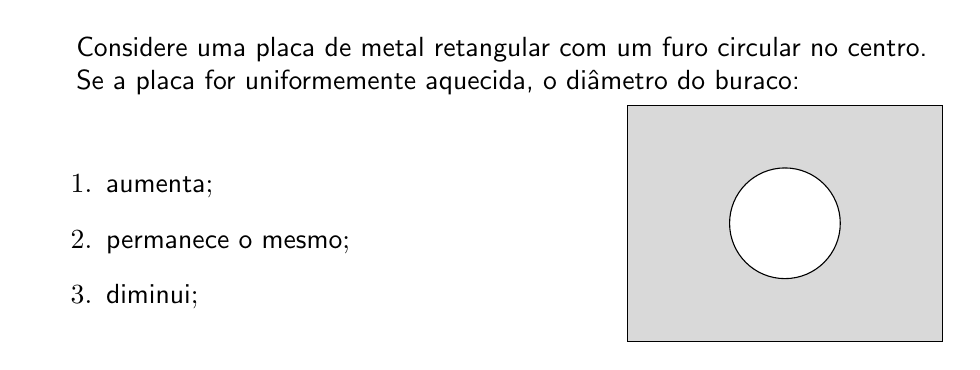
\begin{tikzpicture}[scale=1]
    \label{fig:desenv_ct}
    \node[,text width=11cm] at (0,4) {\textsf{Considere uma placa de metal retangular com um furo circular no centro. Se a
    placa for uniformemente aquecida, o diâmetro do buraco:}};
    \node[,text width=5cm] at (-3.5,2) {
      \begin{enumerate}
        \item \textsf{aumenta};
        \item \textsf{permanece o mesmo};
        \item \textsf{diminui};
      \end{enumerate}
    };
    \draw[fill=gray!30, shift={(1.5cm,.5cm)}](0,0) rectangle (4,3);
    \draw[fill=white, shift={(1.5cm,.5cm)}](2,1.5) circle(20pt);
  \end{tikzpicture}
  \fonte{Adaptado de \cite{Watkins2013}}
\end{figure}

Uma das etapas do IpC na sala de aula é o processo de votação, como mencionado
anteriormente. Existem pelo menos quatro maneiras \cite{Crouch2007} do professor
obter um \textit{feedback} da classe:

\begin{description}
  \item[Levantar as mãos] a forma mais simples é pedir para os alunos levantarem as mãos para cada alternativa,
  mas dentre as várias limitações desse método temos que os estudantes podem se
  influenciar pela resposta dos outros.
  \item[Cartões coloridos] uma segunda alternativa seria o uso de
  cartões coloridos (\textit{flashcards}) que dificultaria os alunos ver a resposta
  dos outros e facilitaria a contagem pelo professor, porém uma limitação desse método,
  assim como o anterior é a dificuldade de alguma forma guardar os resultados.
  \item[Folha de respostas] outra alternativa, no entanto não seria possível ter
  um resultado imediato das respostas.
  \item[Sistemas de resposta em sala de aula] exemplo os \textit{clickers} da \autoref{fig:desenv_clickers}, ou \textit{smartphones},
  e sistemas web possibilitam aos estudantes enviarem imediatamente as respostas ao
  computador do professor, de forma anônima aos colegas de sala e visualizar graficamente
  os resultados.
\end{description}

% 1) a forma mais simples é pedir para os alunos levantarem as mãos para cada alternativa,
% mas dentre as várias limitações desse método temos que os estudantes podem se
% influenciar pela resposta dos outros, 2) uma segunda alternativa seria o uso de
% cartões coloridos (\textit{flashcards}) que dificultaria os alunos ver a resposta
% dos outros e facilitaria a contagem pelo professor, porém uma limitação desse método,
% assim como o anterior é a dificuldade de alguma forma guardar os resultados,
% 3) folha de respostas seria outra alternativa, no entanto não seria possível ter
% um resultado imediato das respostas, 4) já sistemas de resposta em sala de aula como
% os \textit{clickers} da \autoref{fig:desenv_clickers}, ou \textit{smartphones},
% e sistemas web possibilitam aos estudantes enviarem imediatamente as respostas ao
% computador do professor, de forma anônima aos colegas de sala e visualizar graficamente
% os resultados \cite{Crouch2007}.


\begin{figure}
  \begin{centering}
    \caption{\label{fig:desenv_clickers}Exemplo de \textit{clickers}}
    \subfloat[\textit{i>clicker 2}]{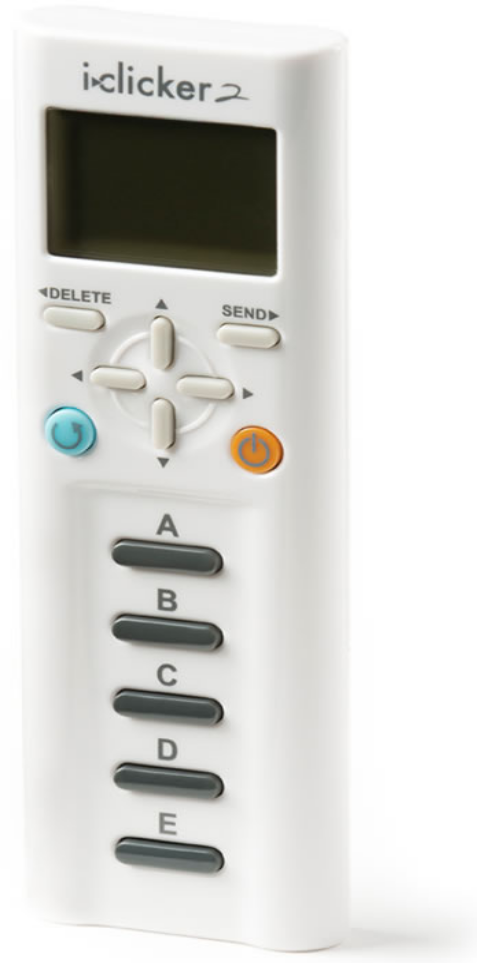
\includegraphics[scale=0.25]{imagens/desenv_iclicker}\label{fig:clickersA}}
    \hspace{.5cm}
    \subfloat[\textit{ResponseCard RF LCD}]{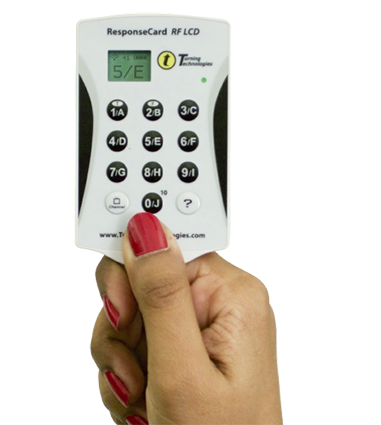
\includegraphics[scale=.4517]{imagens/desenv_turning_clicker}}
    \par
  \end{centering}
  \fonte{(a) \href{http://www1.iclicker.com}{iclicker.com} (b) \href{http://www.turningtechnologies.com}{turningtechnologies.com}}
\end{figure}

No entanto, a implementação do IpC não ocorre apenas na sala de aula. Espera-se
que os alunos façam leituras e atividades antes da aula. Também espera-se do
professor guiar os estudantes nessa etapa, seja indicando ou disponibilizando o
material adequado. O tempo em sala de aula que seria utilizado para apenas transferir
informações para os estudante é utilizado principalmente para discussões, interação
entre os estudantes, tempo para assimilação e para pensar \cite{Mazur2009, Crouch2001}.

\begin{figure}[htbp]
  \centering
  \caption{Diagrama do processo de implementação do método IpC}
  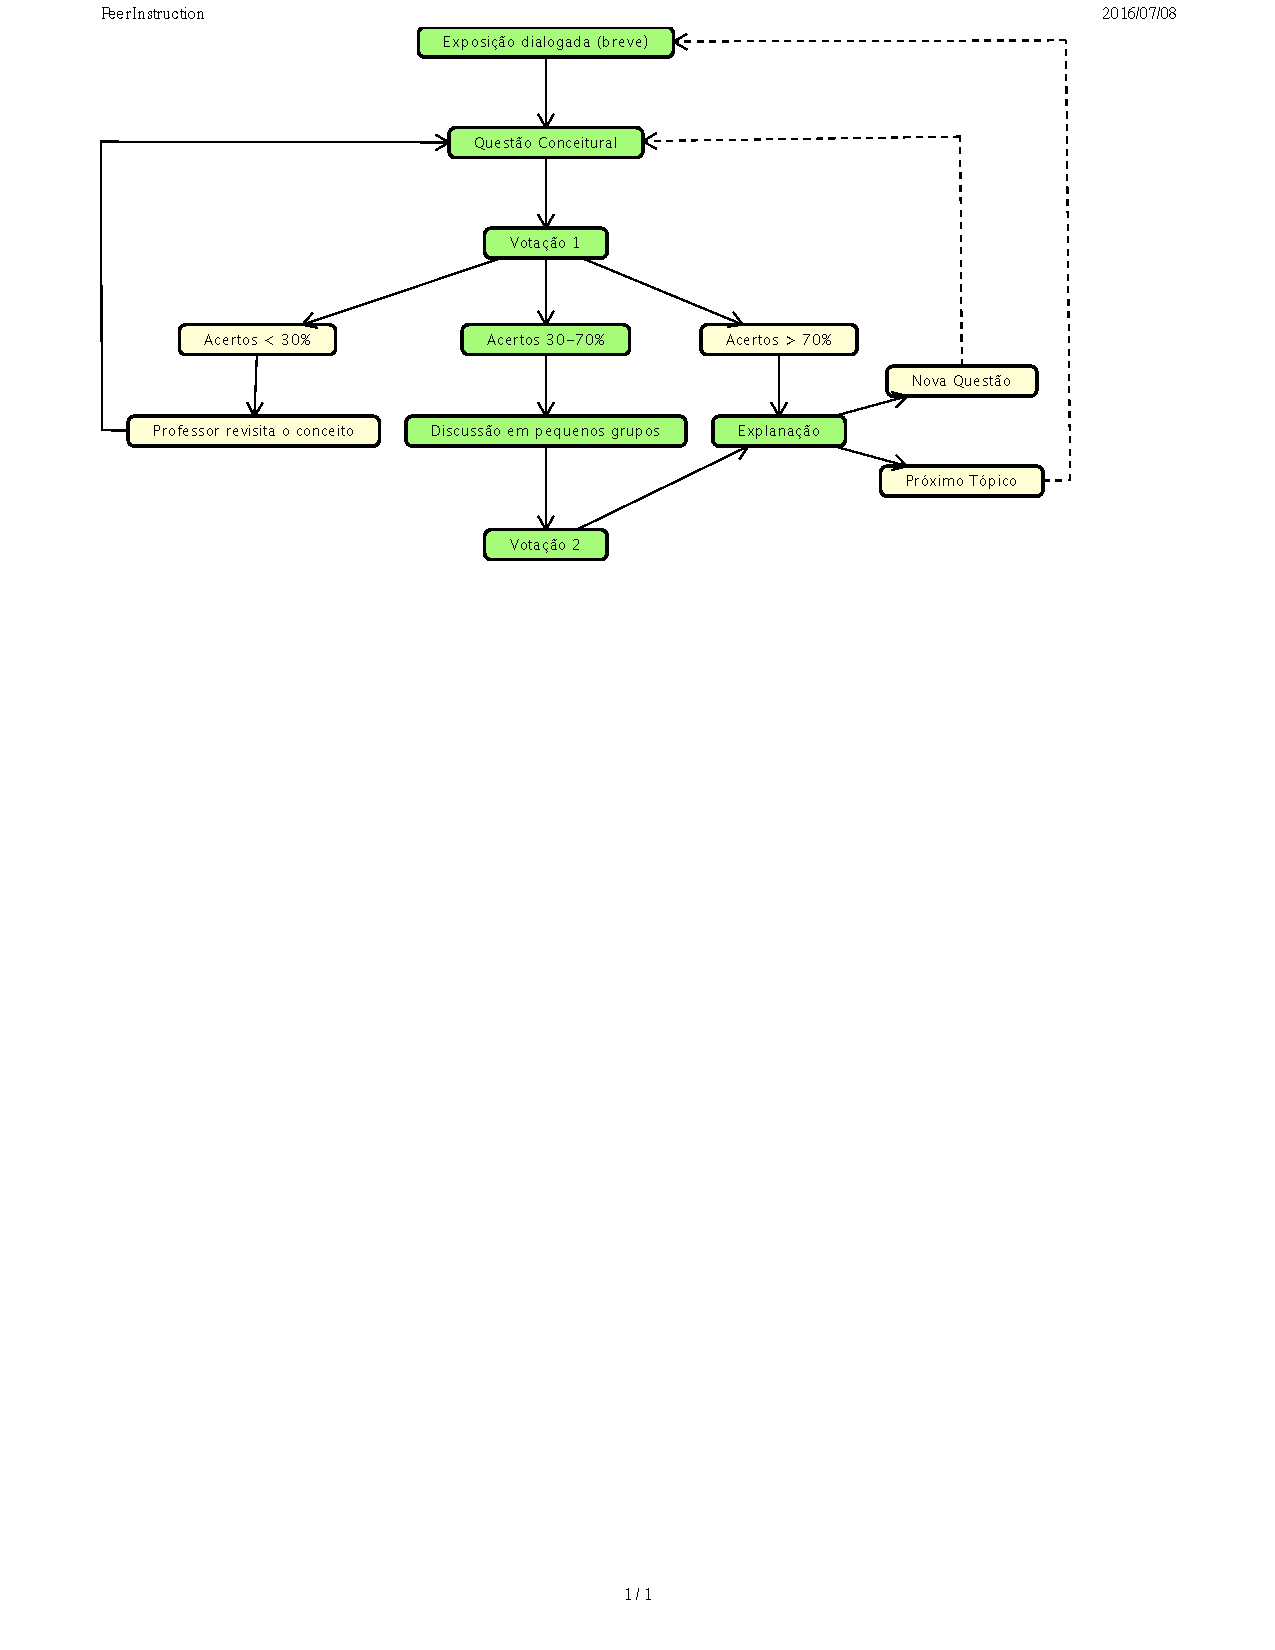
\includegraphics[clip, trim=0cm 18cm 3cm .4cm, width=.85\textwidth]{imagens/peer_instruction}
  \label{fig:desen_fluxograma_ipc}
  \fonte{Adaptado de \cite{Araujo2013}}
\end{figure}


\section{Sistemas de Resposta em Sala de Aula}
\label{section:sistemas_de_resposta}

Sistemas de respostas em sala de aula são tecnologias que permitem ao professor
realizar questionamentos a toda classe e assim obter o resultados das respostas
em tempo real \cite{Kay2009}. Geralmente, as questões são no formato de verdadeiro ou
falso e questões de múltipla escolha. Tais sistemas também podem ser usados para
saber a impressão dos alunos sobre determinado tema \cite{Fies2006}.

Inicialmente introduzido em 1966 na Universidade de Stanford (EUA), os sistemas
de resposta não funcionavam direito, eram difíceis de usar e caros \cite{Kay2009}. Dispositivos
como os da \autoref{fig:desenv_clickers} que usam infravermelho, com preços mais
atrativos, começaram a ser extensivamente usados a partir de 2003 e hoje existe pelo
uma disciplina em cada universidade dos Estados Unidos em que se faz uso de tais sistemas
no processo de ensino e aprendizagem \cite{Abrahamson2014}.

Entretanto, ainda que o custo individual de um aparelho seja atrativo para um
estudante, a realidade da universidade pública brasileira é diferente em relação
a dos Estados Unidos. Assim como não existe obrigatoriedade do aluno comprar um
livro-texto no Brasil, também não existe mecanismo que os faça
comprar \textit{clickers} \cite{GerdKortemeyerEmersonCruz2011}. Dessa forma, os \textit{clickers}
teriam que ser comprados pela universidade, e o custo total não seria tão atrativo.

Por exemplo, a Universidade de São Paulo (USP)\nomenclature{USP}{Universidade de São Paulo}, em uma tentativa pioneira de
\citeonline{GerdKortemeyerEmersonCruz2011} de oferecer oportunidades para avaliação
formativa usando \textit{clickers} como os da \autoref{fig:clickersA} em duas
turmas de física com 80 alunos cada. Com cada \textit{i>clicker 2}
custando \$43,74 (\textit{vide} \autoref{fig:desenv_preco})
o valor total apenas dos 160 \textit{clickers} seria de
R\$22.116,34\footnote{Considerando o valor do dólar comercial em 12. Ago. 2016
de R\$3,1602. Disponível em: \href{http://www4.bcb.gov.br/pec/taxas/port/ptaxnpesq.asp?id=txcotacao}{http://www4.bcb.gov.br/pec/taxas/port/ptaxnpesq.asp?id=txcotacao}},
necessitando ainda do aparelho que recebe as respostas, software que é instalado
no computador do professor, treinamento e suporte, ou seja, o valor final pode ser
ainda maior. A propósito, essa é uma das principais barreiras na adoção dessa
ferramenta no processo de ensino, que ainda tem a resistência de alguns professores
em usar novas tecnologias como ferramentas de ensino \cite{Moratelli2014, Blasco-Arcas2013, Strasser2010, GerdKortemeyerEmersonCruz2011, Kay2009}.

\begin{figure}[!t]
  \centering
  \caption{Preço do \textit{i>clicker 2}}
  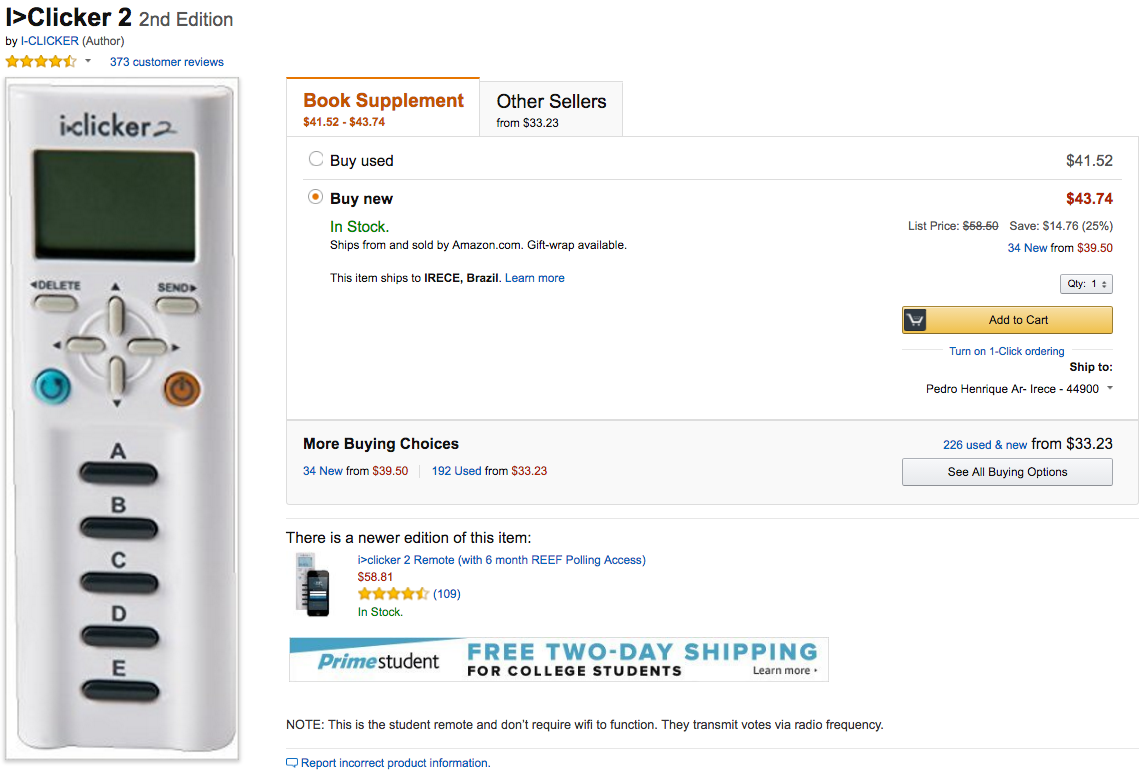
\includegraphics[width=.75\textwidth]{imagens/desenv_preco}
  \fonte{\href{https://goo.gl/q4nBdg}{amazon.com} pesquisando \textit{i>clicker 2}. Acesso em 12. Ago. 2016}
  \label{fig:desenv_preco}
\end{figure}

Todavia, uma maneira de tornar tal tecnologia mais acessível é usar os próprios
celulares dos estudantes como {\clickers} \cite{Stowell2015, Morrell2015, Araujo2013}.
Além de mais acessível, usando os próprios celulares, os estudantes podem
ver as questões e os resultados da classe nos próprios aparelhos. Para o professor,
uma variedade maior de questões podem ser exploradas, como uma  questão aberta \cite{Stowell2015}.

Saliente-se ainda que, embora possa haver um pequeno aumento no número de questões
sem respostas, as respostas dos estudantes são comparáveis quando se usa
\textit{clickers} \cite{Morrell2015, Stowell2015}.

Ainda que o uso do celular como {\clicker} possa aumentar o nível de
distrações, são muitos os benefícios de usar essa abordagem, no entanto,
é preciso estar atento aos pequenos casos de estudantes que não têm a tecnologia
adequada, ou que não queiram usar os seus dispositivos \cite{Morrell2015, Stowell2015}.

\subsection{\textit{Smartphones} no Brasil}

É importante aqui destacar o uso dos dispositivos que podem permitir essa abordagem
na realidade brasileira. Hoje existem 1,2 dispositivos portáteis
(\textit{smartphones} e \textit{tablets}) por habitante e uma projeção para o próximo
biênio 2017/2018 de 2 dispositivos
(desktops, \textit{notebooks}, \textit{tablets} e \textit{smartphones}) por habitante \cite[p. 8]{Meirelles2016}.
Acrescenta-se também que já em 2014 mais de 93\% dos estudantes da rede privada de
ensino e quase 67\% dos da rede pública possuem \textit{smartphones}, em que a
proporção de pessoas é maior na rede pública \cite[p. 55]{IBGE2016}. Também cabe
ressaltar que o celular já é o principal meio para acessar a Internet nos domicílios
brasileiros \cite[p. 41]{IBGE2016}.

\subsection{Alternativas Disponíveis}
\label{subp:alternativas_disponiveis}

Cabe a este respeito apresentar algumas soluções disponíveis que permitem usar o celular como
{\clicker}.

Em um estudo para desenvolver uma estratégia de ensino utilizando
{\clickers} como recurso didático \citeonline{Mattos2015}, utilizou o
\href{https://www.polleverywhere.com/}{\textit{Poll Everywhere}} que foi
escolhido principalmente por ser compatível com as principais plataformas
móveis (Android, iOS e Windows Phone). O
\href{https://www.polleverywhere.com/}{\textit{Poll Everywhere}} oferece uma
versão gratuita com no máximo 40 respostas por votação com algumas limitações.
Na versão paga, o estudante pode pagar \$14/ano ou o professor pode pagar
\$349/semestre (vide \autoref{fig:polleverywhere}).

Outra solução é o \href{http://www.socrative.com/}{\textit{Socrative}},
que também é compatível com todas as plataformas, e na sua versão gratuita
permite até 50 alunos por votação, questões de múltipla escolha, de verdadeira e falso,
resposta curta, \textit{quizzes}, etc \cite{socrative2016}. Alguns relatos do uso do
\href{http://www.socrative.com/}{\textit{Socrative}} em sala de aula para promover
a interatividade são encontrados em \cite{Kaya2016, Trindade2014}.
Uma opção interessante do \href{http://www.socrative.com/}{\textit{Socrative}}
é o \textit{Exit Ticket}, em que ao final da aula os estudantes respondem
a três perguntas. A primeira funciona como uma autoavaliação, perguntando
o quanto o estudante entendeu da aula, já as outras duas como identificação, que são o
nome do aluno e uma pergunta que o professor coloca no quadro, ou seja, teoricamente,
apenas os alunos presentes vão ser capazes de responder corretamente, servindo
então como um controle de frequência. Na versão paga o professor pode pagar \$49,99/ano (vide \autoref{fig:socrative}).

Por último, o aplicativo \href{http://www.tophat.com/}{\textit{TopHat}}, que parece
ser usado diariamente por mais 500 instituições de ensino pelo mundo \cite{tophat2016}.
Para o professor, \href{http://www.tophat.com/}{\textit{TopHat}} permite incorporar
uma variedade de questões, também uma revisão interativa da aula e para provas
\cite{Neilson2016, Lantz2014}. A inscrição mais popular no  \href{http://www.tophat.com/}{\textit{TopHat}}
são de \$36/ano (vide \autoref{fig:tophat}).

\begin{figure}
  \centering
  \caption{Preço de algumas sistemas de resposta}
  \subfloat[Disponível em: \href{https://www.polleverywhere.com/plans/higher-ed}{polleverywhere.com/plans/higher-ed}: em 16 ago. 2016]{
    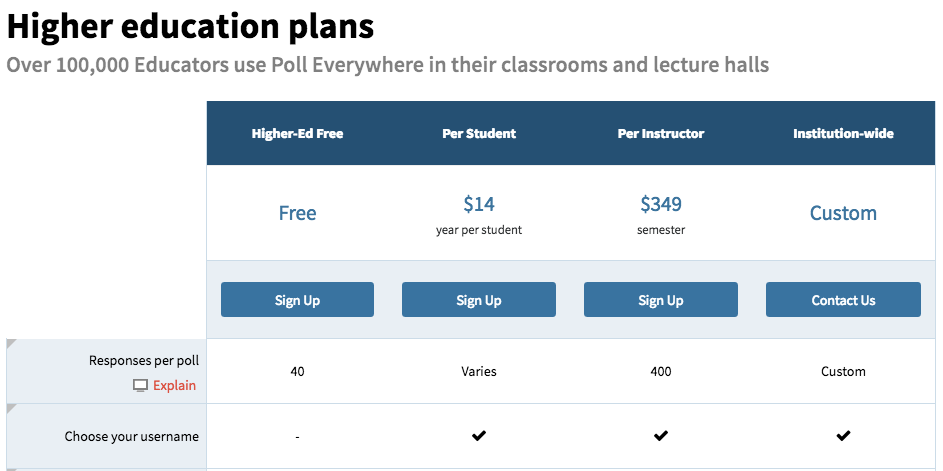
\includegraphics[scale=0.35]{imagens/polleverywhere2}
    \label{fig:polleverywhere}
  }

  \subfloat[Disponível em: \href{http://www.socrative.com/pricing.php}{socrative.com/pricing}: em 16 ago. 2016]{
    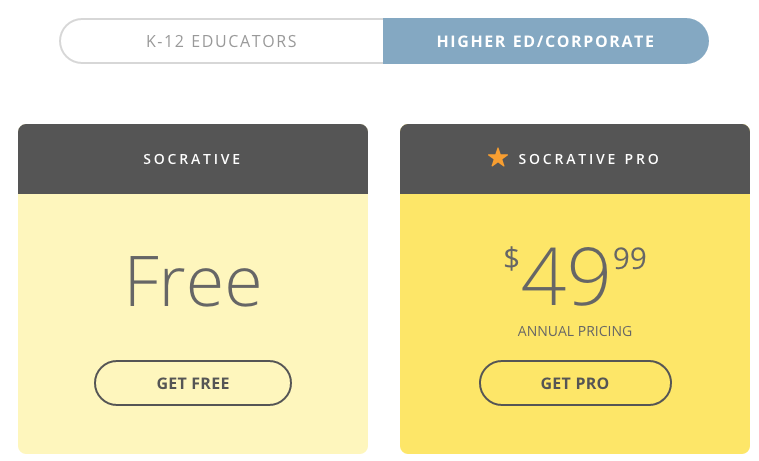
\includegraphics[scale=0.35]{imagens/socrative}
    \label{fig:socrative}
  }

  \subfloat[Disponível em: \href{https://tophat.com/pricing/}{tophat.com/pricing} em: 16 ago. 2016]{
    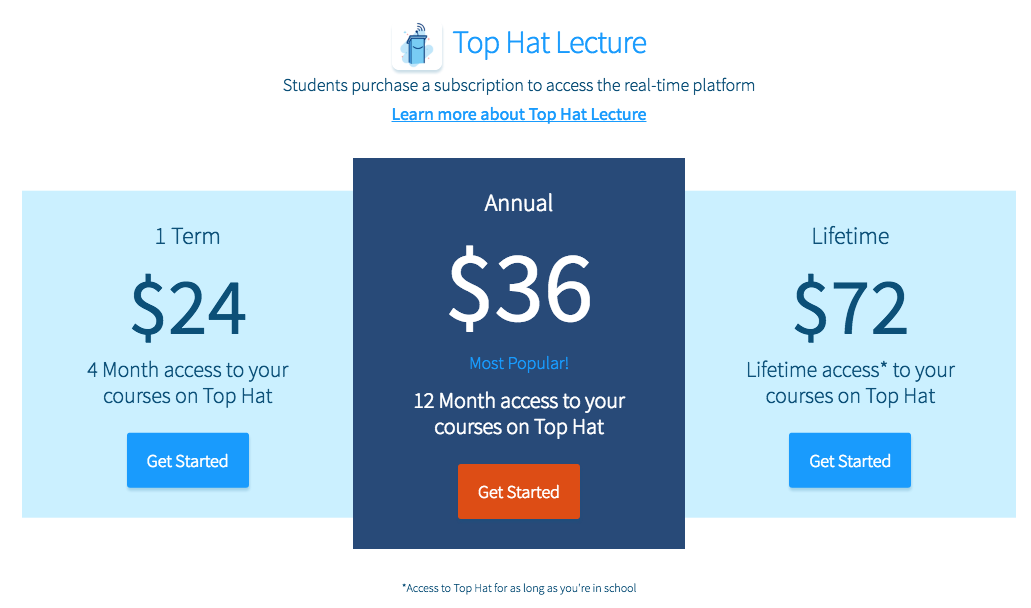
\includegraphics[scale=0.35]{imagens/tophat}
    \label{fig:tophat}
  }
\end{figure}

\section{Benefícios dos Sistemas de Resposta em Sala de Aula}
Os benefícios do uso de sistemas de resposta em sala de aula podem ser divididos
em benefícios para a sala de aula, para a aprendizagem e para avaliação \cite{Kay2009}. As
subseções a seguir discutem cada tópico.

% Com efeito, a tecnologia apresenta-se como meio, como instrumento para colaborar no desenvolvimento do processo de aprendizagem.
% A tecnologia reveste-se de um valor relativo e dependente desse processo. Ela tem sua importância apenas como um instrumento significativo para favorecer a aprendizagem de alguém. Não é a tecnologia que vai resolver ou solucionar o problema educacional do Brasil. Poderá colaborar, no entanto, se for usada adequadamente, para o desenvolvimento educacional de nossos estudantes.

Por outro lado, apesar das seções a seguir serem animadoras quanto ao uso dos
{\clickers} é importante destacar a tecnologia apenas como um meio para
colaborar no processo de ensino e aprendizagem, e só faz sentido quando associada
com práticas pedagógicas de ensino como o aprendizado ativo
(vide \autoref{section:aprendizado_ativo}) \cite{Terrion2012, Moran2006}. O leitor interessado
sobre o uso das novas tecnologias em sala de aula, poderá buscar nas obras
indicadas em \cite{portalBrasil2014}.

Realmente, na mais recente revisão de literatura sobre {\clickers} desde \cite{Kay2009},
\citeonline{Han2014} concluiu que o ensino e aprendizado com o auxílio de {\clickers}
ainda é um fenômeno complexo e relacional. Segundo o mesmo autor, estudos mais rigorosos
devem ser conduzidos para se entender por exemplo a relação entre o uso de {\clickers}
e o aprendizado, pois o benefícios da tecnologia podem variar pelo histórico do
estudante, motivação e metacognição.

\subsection{Benefícios para a sala de aula}

\subsubsection{Frequência Escolar}
Não apenas uma ferramenta que também pode facilitar o controle de frequência
\cite{Strasser2010},
os sistemas de resposta em sala de aula têm sido utilizados com sucesso para aumentar
a frequência escolar \cite{Fotaris2016, Velasco2013, Puente2012, Mayer2009, Caldwell2007}. O fato dos
estudantes terem tido um retorno imediato das atividades que faziam interativamente
na sala de aula, pode ter contribuído para motivar os alunos para irem para as aulas \cite{Puente2012}.
Outro fator para o aumento da frequência é quando as questões dos {\clickers} contribuem na nota final,
em que o peso pode variar de 5\% a 15\% que o resultado parece ser o mesmo \cite{Caldwell2007}.

\subsubsection{Atenção}\label{subsubsection:attention}
Sabe-se hoje que a maioria das pessoas não conseguem se concentrar ininterruptamente
por mais de 20 min em uma única atividade \cite{Caldwell2007, DInverno2003}. Com aulas que
duram entre 2h-3h, os professores podem quebrar as aulas em miniaulas
com questões ao final delas usando os {\clickers} \cite{Hunsu2016}. Estudo de
ondas cerebrais mostraram que a atenção dos estudantes aumentam durante as
atividades de votação, além de reduzir a ansiedade \cite{Sun2014}. Acrescenta-se
também que quando os {\clickers} são adotados, os estudantes relatam a necessidade
de estudar antes da aula para participarem e prestarem atenção, dessa forma participam mais da aula \cite{Terrion2012}.

\subsubsection{Privacidade e Participação}\label{subsubsection:privacy}
Os estudantes podem responder as questões sem se preocupar com o julgamento
de seus colegas de classe ou do professor. Nesse ambiente seguro o estudante
não tem nenhuma razão para sentir medo de responder errado \cite{Schmidt2011}.
 A falta de privacidade pode coibir
a completa honestidade na votação \cite{Caldwell2007}, e a presença da mesma da a oportunidade
para os estudantes responderem e tomarem posições polêmicas em questões sensíveis \cite{Rana2016}.

\subsubsection{Engajamento}
Inúmeros estudos indicam estudantes mais interessados ou engajados no material
apresentado quando sistemas de resposta são usados
\cite{Kaya2016, Rana2016, Horne2015, Mattos2015, Moratelli2014, Kulatunga2014, Blood2013, Terrion2012,
Caldwell2007}.

\subsection{Benefícios para a aprendizagem}

\subsubsection{Interação e Discussão}
A interação na sala de aula é importante por três motivos: primeiro pelo que foi
apresentado na \autoref{subsubsection:attention}, segundo que permite clarificar
pontos obscuros e terceiro que permite uma monitoração do entendimento da classe
e velocidade do que é apresentado \cite{DInverno2003}. Nesse sentido, estudos
indicam aumento da interação na sala de aula \cite{Mattos2015, Barragues2011, Titman2011, Mayer2009, Caldwell2007}.

\subsubsection{\textit{Contingent Teaching}}\label{sussubsection:contingent}
\textit{Contingent Teaching} nada mais é do que a possibilidade de modificar
o curso do que está sendo ensinado baseado no \textit{feedback} dos estudantes
\cite{Arnesen2013, Caldwell2007}. Por exemplo, se pouco mais da metade da classe
responde corretamente a uma questão, conclui-se uma falta de compreensão geral do
tópico apresentado, e assim o professor pode tentar explicar o conceito
de maneira diferente \cite{Terrion2012, Strasser2010}.

\subsubsection{Melhora no aprendizado}
\citeonline{Lantz2014} verificaram um aumento significativo (15\%) no grupo de
participantes que tiveram aulas com {\clickers} daqueles sem o uso em testes que
ocorriam dois dias depois as aulas, e também permitiu aos estudantes corrigir
eventuais equívocos sobre o material de aula. Outros estudos apontam melhora
na performance \cite{Sun2014, Caldwell2007}. Entretanto, em um recente estudo de meta-análise,
em que se comparou classes que usaram e não usaram sistemas de resposta em sala de aula,
indicou um pequeno mas significativo impacto positivo nas variáveis cognitivas (retenção,
transferencia de conhecimento e sucesso), e de pequeno para médio no que se refere
as variávies não-cognitivas (engajamento e participação, frequência, interesse,
percepção de qualidade) \cite{Hunsu2016}.

\subsection{Benefícios para avaliação}

\subsubsection{\textit{Feedback}}
Como destacado na \autoref{section:ipc}, dentre as quatro formas disponíves para
o professor obter um \textit{feedback} ou retorno do entendimento dos estudantes
sobre determinado tópico, se disponível, os {\clickers} são os mais eficazes \cite{Crouch2007}.
Os {\clickers} permitem um retorno imediato, preciso, privacidade (vide \autoref{subsubsection:privacy}) e
são divertidos de usar \cite{Rana2016, Blood2013, Caldwell2007}.

\subsubsection{Avaliação Formativa}
Avaliar o estudante permanemtemente, e não apenas utilizando avaliações pontuais,
não apenas classificar os alunos em os que sabem e os que não sabem, não apenas
verificar e sim avaliar, dedicar mais tempo nos erros \cite{UnivespTV2013}. Esses são alguns pontos
da avaliação formativa, que para o professor orienta a prática pedagógica, e para
o aluno permite uma autoavaliação sobre a aprendizagem \cite{Kay2009}. Os artigos
a seguir indicam que o uso de sistemas de resposta em sala de aula ajudam a
fornecer avaliações formativas eficazes \cite{Kortemeyer2016, Thampy2014, Kay2009, Fies2006}.

\subsection{Desafios para usar {\clickers}}
O uso dos {\clickers} também trazem alguns desafios, principalmente
de tecnológicos ou estruturais e desafios centrado nos estudantes \cite{Cubric2015, Kay2009}.

\subsubsection{Tecnológicos/Estruturais}
\citeonline{Stowell2015} recomenda que as salas de aula tenham acesso confiável
a rede Wi-Fi, por isso o professor deve estar preparado quando a internet não
estiver disponível \cite{Strasser2010}. Como já abordado nesse trabalho (vide \autoref{section:sistemas_de_resposta}),
nem todos os estudantes vão ter a tecnologia adequada ou vontade de usar \cite{Morrell2015, Stowell2015}.
Dessa forma, \citeonline{Velasco2013} aconselham os {\clickers} como uma ferramenta opcional para
os estudantes.

\subsubsection{Desafio para os estudantes}
Alguns estudantes podem ter resistência ao novo, principalmente se já acomodados
a passividade em sala de aula \cite{Terrion2012, Kay2009}. Além disso, quando
usados apenas para controle de frequência, os estudantes podem ter uma percepção
negativa da tecnologia \cite{Terrion2012, Caldwell2007}.
